\documentclass[11pt,a4paper]{article}
\usepackage{diagbox}
\usepackage{wrapfig}
\usepackage[utf8]{inputenc}
%\usepackage[swedish]{babel}
\usepackage{graphicx}
\usepackage{amsmath}
\usepackage{amssymb}
\usepackage{units}
\usepackage{ae}
\usepackage{icomma}
\usepackage{xcolor}
\usepackage{graphics}
\usepackage{bbm}
\usepackage{float}
\usepackage{siunitx}
\usepackage[font={small,it}]{caption}
\usepackage{subcaption}

\usepackage{hyperref}
\usepackage{epstopdf}
\usepackage{epsfig}
\usepackage{braket}
\usepackage{pdfpages}
\usepackage{tcolorbox}
\usepackage{url}
\usepackage{svg}
\usepackage{physics}
% \usepackage{tikz}
% \usepackage{pgfplots}
% \pgfplotsset{compat=newest}
% \usepgfplotslibrary{groupplots}
% \usepgfplotslibrary{dateplot}

\newcommand{\N}{\ensuremath{\mathbbm{N}}}
\newcommand{\Z}{\ensuremath{\mathbbm{Z}}}
\newcommand{\Q}{\ensuremath{\mathbbm{Q}}}
\newcommand{\R}{\ensuremath{\mathbbm{R}}}
\newcommand{\C}{\ensuremath{\mathbbm{C}}}
\newcommand{\id}{\ensuremath{\,\mathrm{d}}}
\newcommand{\rd}{\ensuremath{\mathrm{d}}}
\newcommand{\Ordo}{\ensuremath{\mathcal{O}}}% Stora Ordo
\renewcommand{\L}{\ensuremath{\mathcal{L}}}% Stora Ordo
\newcommand{\sub}[1]{\ensuremath{_{\text{#1}}}}
\newcommand{\ddx}[1]{\ensuremath{ \frac{\partial}{\partial #1} }}
\newcommand{\ddxx}[2]{\ensuremath{ \frac{\partial^2}{\partial #1 \partial #2} }}
%\newcommand{\sup}[1]{\ensuremath{^{\text{#1}}}}
\newcommand*\diff{\mathop{}\!\mathrm{d}}
\renewcommand{\vec}[1]{\boldsymbol{#1}}
\renewcommand{\b}[1]{\ensuremath{ {\bf #1 } }}
\renewcommand{\arraystretch}{1.5}

\title{Effect of toroidicity on runaway generation\\\vspace{.3cm} \large{project course FUF060 in plasma physics}}
\author{Peter Halldestam}
\date{\today}

\begin{document}

\maketitle

\abstract{\noindent In a plasma, \textit{runaway electrons} (RE) are created when the force from the macroscopic electric field is greater than the drag force due to collisions with other particles in the plasma.
This results in an acceleration of electrons to extremely high velocities which in turn may damage components of the fusion reactor facing the plasma.
In this report we consider the cross sectional shape of the magnetic field and study its effect on RE generation using the newly developed \textsc{DREAM} \cite{DREAM}.}

\section{Parametrisation of the toroidal magnetic field}
\label{sec:param}
The simulation framework \textsc{DREAM} (\textit{Disruption and Runaway Electron Avoidance Model}) evolves bounce averaged equations of motion in a static magnetic geometry.
Any flux surface labeled $r$ is parametrized by its major radius $R_0$, elongation $\kappa(r)$, triangularity $\delta(r)$ and Shafranov shift $\Delta(r)$.
The three latter and the minor radius $a$ are illustrated in fig.\ \ref{fig:toroidicity}.
Firstly, the elongation is a scale factor determining the ellipticity of the flux surface.
Here, we set a constant $\kappa(r)=\kappa_0$, but it can in general be any positive function of $r$.
The triangularity $\delta(r)$ determines the horizontal shift of the top/bottom-most point of the flux surface and finally, the Shafranov shift $\Delta(r)$, which is the shift from the magnetic axis of the center of a flux surface.
Both the triangularity and Shafranov shift are set to be linear functions $\delta(r)=\delta_0 r/a$ and $\Delta(r)=\Delta_0 r/a$ respectively.
For instance, the configuration $(\kappa_0, \delta_0, \Delta_0)=(1, 0, 0)$ yields a circular cross section with concentric flux surfaces, which is used as the baseline geometry in secs.\ \ref{sec:dreicer} and \ref{sec:avalanche}.

Any position $\vec{x}$ is parametrized with the coordinates $(r, \theta)$ by defining $\vec{x}=R\vec{\hat{R}}+z\vec{\hat{z}}$, where
\begin{align}
    \label{eq:param}
    \begin{cases}
        R
        =R_0+\Delta(r)+r\cos\{\theta+\delta(r)\sin\theta\},\\
        z
        =r\kappa(r)\sin\theta.
    \end{cases}
\end{align}
With this parametrisation, each flux surface is identified by keeping $r$ constant given the major radius of the magnetic axis $R_0$ and the three shaping parameters.\\

\noindent
Furthermore, any arbitrary axisymmetric magnetic field can be expressed as
\begin{align*}
    \vec{B}
    =G\grad{\varphi}+\frac{1}{2\pi}\grad{\varphi}\cross\grad{\psi},
\end{align*}
where $\varphi$ denotes the toroidal angle about which the field is symmetric, $G$ describes the toroidal magnetic field and $\psi$ is the poloidal magnetic flux.
% The latter two are set in accordance to an example in \cite{DREAM} (REFERERA BÄTTRE)
% \begin{align*}
%     G(r)
%     &= B_0 R_0\\
%     \psi(r)
%     &=-\mu_0 I_\text{ref} \bigg[1-\bigg(\frac{r}{a}\bigg)^2\bigg] a
% \end{align*}
For our purposes, the toroidal term will dominate and therefore a useful approximation of the field strength is given by
\begin{align}
    \label{eq:magnetic}
    B
    \approx\frac{B_0 R_0}{R}
    =\frac{B_0 R_0}{R_0+r}
\end{align}
where $B_0=\SI{5}{T}$ is a prescribed value of $B=\abs{\vec{B}}$ at the major radius, ie.\ at $r=0$.
In the simulations, the major and minor radius are set to $R_0=\SI{0.68}{m}$ and $a=\SI{0.22}{m}$ respectively.
\begin{figure}[H]
    \centering
    \captionsetup{width=.8\textwidth}
    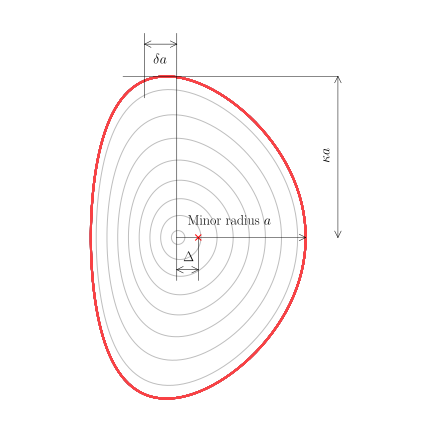
\includegraphics[scale=.7 ]{figs/toroidicity.eps}
    \caption{Tokamak cross section illustrating the three shaping parameters used to define the shape of the magnetic field: elongation $\kappa$, triangularity $\delta$ and Shafranov shift $\Delta$.
    This image is taken from \cite{DREAM}.}
    \label{fig:toroidicity}
\end{figure}

\newpage
\section{Runaway electrons}
Consider a single electron with velocity $v$ in a plasma of both electrons and ions.
The drag force experienced by it scales as $F_\text{drag}\sim m_ev\nu$, where $\nu$ is the collision frequency.
Unlike a regular gas, in which close pair-wise collisions prevail, a plasma is dominated by long range Coloumb interactions.
As a consequence of this, the drag force differs significantly for \textit{cold} and \textit{hot} electrons (ie.\ those with $v\ll v_\text{th}$ or vice versa, where $v_\text{th}$ is the thermal velocity).
The relative velocity as seen by the electron, and thus the collision frequency, is predominantly due to the thermal motion of the surrounding plasma particles for cold electrons.
With the collision frequency $\nu=\nu_\text{th}$ for a thermal plasma and therefore $F_\text{drag}\propto v$.
On the other hand, for hot electrons the relative velocity is dominated by their own velocity $v$ so that $\nu\propto 1/v^3$, and thus $F_\text{drag}\propto 1/v^2$ \cite{vallhagenMSc}.
This behaviour is captured in fig.\ \ref{fig:dragForce}.
\begin{figure}[H]
    \centering
    \captionsetup{width=.8\textwidth}
    \includegraphics[scale=.6]{figs/dragForce.eps}
    \caption{Illustration of the drag force experienced by a electron with velocity $v$ in a plasma with an electric field $E_\parallel$ in magnetic field direction.
    The critical velocity $v_\text{c}$ is marked beyond which the drag force becomes smaller than the accelerating force due to the electric field.}
    \label{fig:dragForce}
\end{figure}
\noindent
Therefore, there must exist a critical speed $v_\text{c}>v_\text{th}$ such that
\begin{align*}
    \pdv{v_\parallel}{t}=-eE_\parallel+F_\text{drag}>0, \quad v>v_\text{c}.
\end{align*}
Here $v_\parallel$ and $E_\parallel$ are the electron velocity and the macroscopic electric field, both projected onto the direction of the magnetic field.
These are accelerated towards the speed of light, hence the name runaways.
As the plasma strives to maintain thermal equilibrium, this gap in the electron distribution will continuously be refilled as slower electrons diffuse into the $v>v_\text{c}$ region, which in turn becomes RE's.
This phenomenon is called the \textit{Dreicer mechanism} after Harry Dreicer, who gave the first detailed account on RE's \cite{dreicer1, dreicer2}.

There are other ways of producing RE's without the need of an already existing RE population, known as ''primary'' mechanisms.
In this category we have eg.\ Compton scattering of photons radiating from the neutron activated wall and $\beta$-decay of tritium \cite{hoppePhD}, but these are neglected in this project.
The only primary generation mechanism that is considered is the Dreicer mechanism.

Provided this seed of RE's, the population can be amplified by the ''secondary'' generation mechanism, also called \textit{avalanche multiplication}.
Via large-angle Coloumb collisions of existing runaways with slower electrons such that both end up with a velocity higher than the critical velocity $v_c$, this mechanism leads to an exponential growth of the RE population \cite{vallhagenMSc}. \textcolor{red}{Nåt om hur de förlorar energi också\dots}

In a plasma with a density $n_\text{re}$ of electrons with $v>v_\text{c}$, the rate of which runaways are generated due to these two mechanisms is given by the equation
\begin{align*}
    \dv{n_\text{re}}{t}
    =\gamma+n_\text{re}\Gamma,
\end{align*}
where $\gamma$ is the rate due to the Dreicer mechanism and $\Gamma$ is the avalanche growth rate \cite{hoppePhD}.


During a simulation in \textsc{DREAM}, the program keeps track of the runaway rate as a flux surface averaged quantity
\begin{align*}
    \expval{\dv{n_\text{re}}{t}}
    &=\frac{1}{V'}\int_0^{2\pi}\diff{\varphi}\int_{-\pi}^{\pi}\diff{\theta}\mathcal{J}\dv{n_\text{re}}{t},\\
    V'
    &=\int_0^{2\pi}\diff{\varphi}\int_{-\pi}^{\pi}\diff{\theta}\mathcal{J},\\
    \mathcal{J}
    &=\frac{1}{\abs{\grad{\varphi}\vdot(\grad{\theta}\cross\grad{r})}},
\end{align*}
where $S$ is the area of the surface and $\mathcal{J}$ is the Jacobian of the spatial coordinate system.


In the following sections, we investigate the effect the tokamak geometry have on this flux averaged electron runaway generation individually.
Firstly, without the Avalanche effect included in the simulations and solely focusing on Dreicer generation $\gamma$, we vary the three shaping parameters individually with the baseline geometry being that of a circular plasma cross section with concentric flux surfaces.
Furthermore, we also study the effect the toroidicity $\epsilon=r/R_0$ has on the RE generation to compare with a similar investigation by E.\ Nilsson \textit{et al} \cite{nilsson} which is based on the code \textsc{LUKE}, a solver of the 3D linearized bounce averaged relativistic electron Fokker-Planck equation.
Then we do the same set of studies focusing instead on the avalanche multiplication factor $\Gamma$.

\subsection{Dreicer generation}
\label{sec:dreicer}
In fig.\ \ref{fig:elongation}, the runaway rates from three different simulations with different orders of magnitude in the elongation $\kappa$ are shown to the left and an outlining of their corresponding tokamak cross sections to the right.
The elongation has seemingly no effect on the runaway generation, at least in this range of values.
Out of all three shaping parameters, this seems to be case only for $\kappa$.

Two similar analyses was performed for the triangularity $\delta$ in fig.\ \ref{fig:triangularity} and the Shafranov shift $\Delta$ in fig.\ \ref{fig:shafranovShift}.
Here we observe that cross sections with geometric centres farther away from the center of the tokamak $R=0$ tend to have less runaway electrons generated.

\begin{figure}[H]
    \centering
    \captionsetup{width=.8\textwidth}
    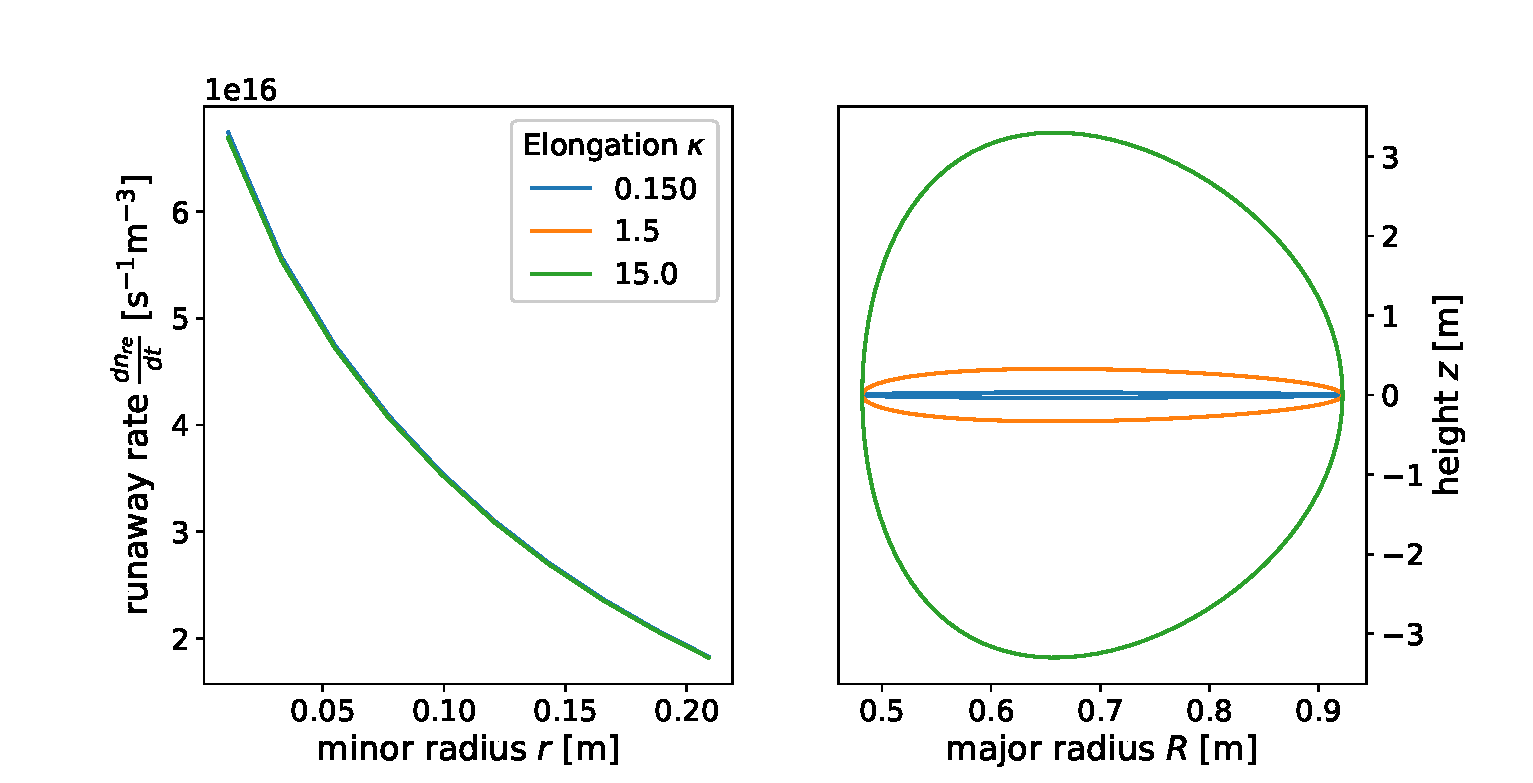
\includegraphics[width=.8\textwidth]{figs/elongation.eps}
    \caption{Flux surface averaged electron runaway rate $\langle\diff{n}_{re}/\diff{t}\rangle$ vs.\ minor radius coordinate $r$ for three different elongations $\kappa$ (left), and corresponding tokamak cross sections (right).
    No significant effect of $\kappa$ on the runaway rate is observed.}
    \label{fig:elongation}
\end{figure}

\begin{figure}[H]
    \centering
    \captionsetup{width=.8\textwidth}
    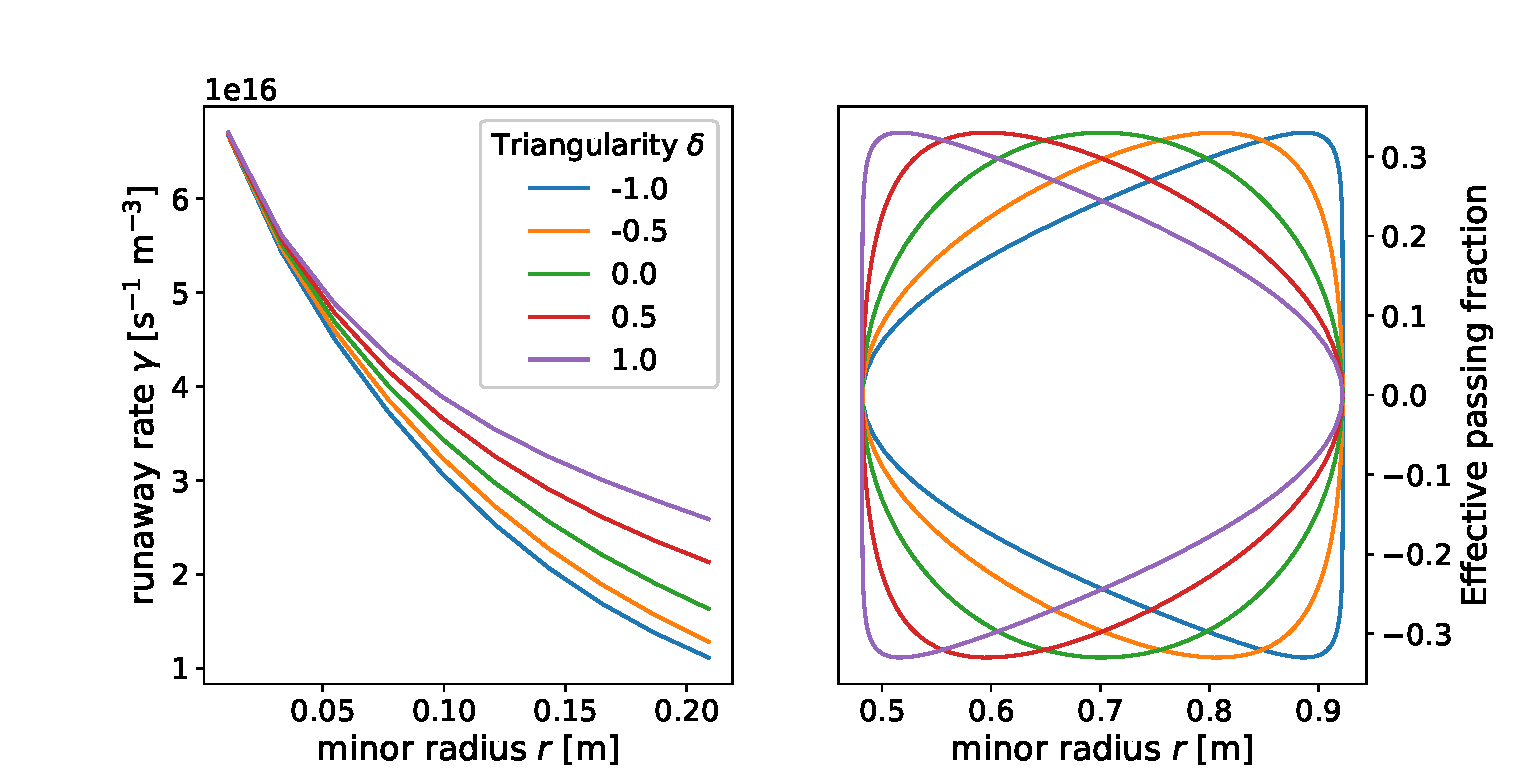
\includegraphics[width=\textwidth]{figs/triangularity.eps}
    \caption{Flux surface averaged electron runaway rate $\langle\diff{n}_{re}/\diff{t}\rangle$ vs.\ minor radius coordinate $r$ for five different triangularity $\delta$ (left), and corresponding tokamak cross sections (right).}
    \label{fig:triangularity}
\end{figure}

\begin{figure}[H]
    \centering
    \captionsetup{width=.8\textwidth}
    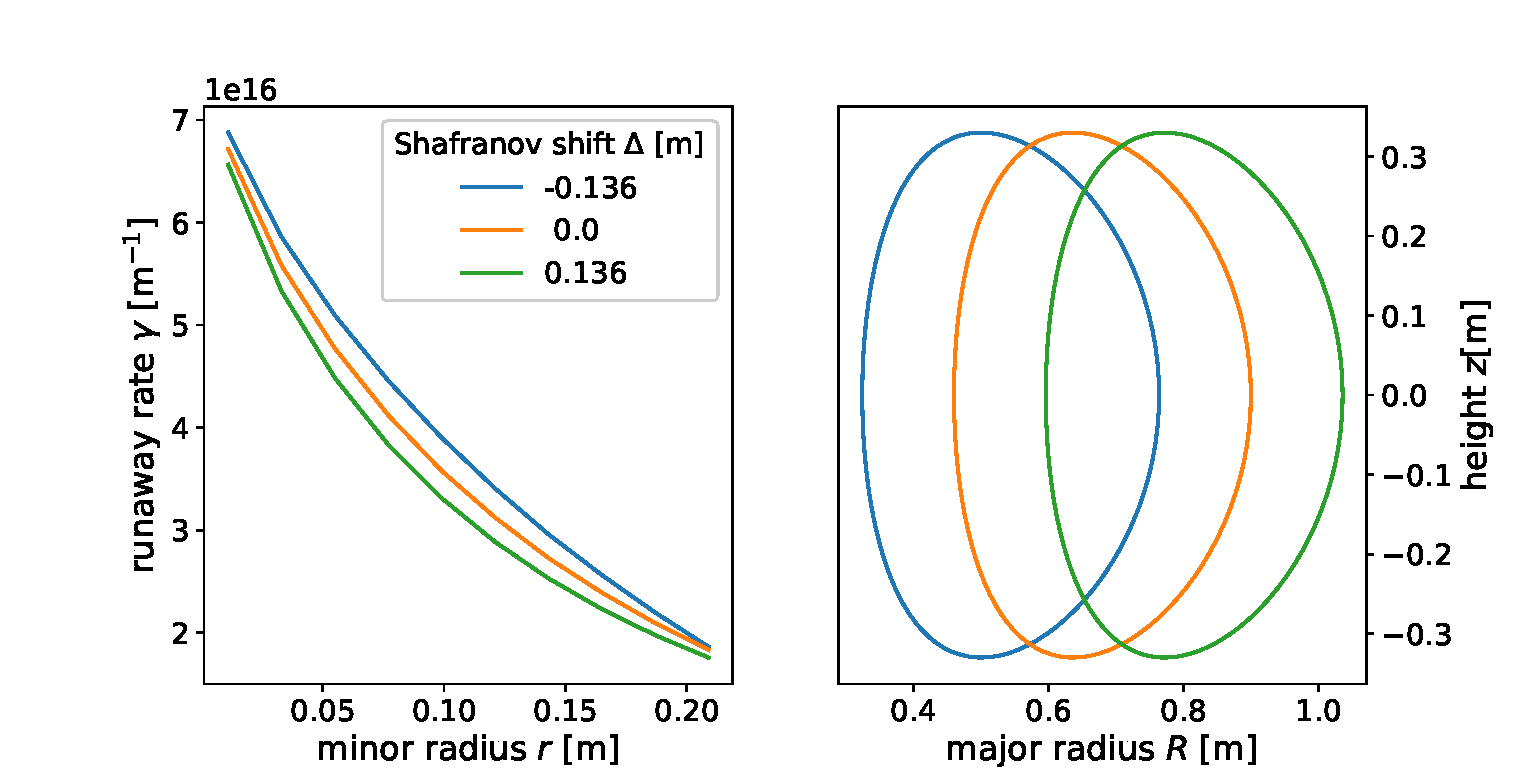
\includegraphics[width=\textwidth]{figs/shafranovShift.eps}
    \caption{Flux surface averaged electron runaway rate $\langle\diff{n}_{re}/\diff{t}\rangle$ vs.\ minor radius coordinate $r$ for three different Shafranov shifts $\Delta$ (left), and corresponding tokamak cross sections (right).}
    \label{fig:shafranovShift}
\end{figure}

\noindent
An explanation for this could possibly be the \textit{magnetic mirror effect} and the concept of \textit{trapped particles}.
Consider a charged particle with velocity components parallel $\vec{v}_\parallel$ and perpendicular $\vec{v}_\perp$ to the magnetic field, starting off at the point of its trajectory where the magnetic field strength is at its lowest $B=B_\text{min}$.
Its guiding center will \textcolor{red}{approximately?} follow a magnetic field surface and along its trajectory, the particle will experience a deaccelerating force as it moves towards higher $B$, namely
\begin{align*}
    m\dv{\vec{v}_\parallel}{t}=-\mu\grad_\parallel{B}.
\end{align*}
Here $\mu=mv_\perp^2/2B$ denotes the magnetic moment, which is an adiabatic invariant.
If the particle ever reaches $v_\parallel=0$, $v_\parallel$ will change sign and it will be forced to turn back.
It is trapped.

One can obtain a condition for a particle to be trapped based on its initial pitch $\xi_0=v_\parallel/v$ when it is at $B=B_\text{min}$ using conservation of energy \cite{hoppeBSc}.
At any time has the total energy
\begin{align*}
    E_0
    =E_\parallel + E_\perp
    =\frac{mv_\parallel^2}{2}+\mu B
\end{align*}
The energies $E_\parallel$ and $E_\perp$ both add up the constant $E_0$, and represents the kinetic energy stored in motion parallel and perpendicular to the magnetic field surfaces respectively.
The particle is trapped if $E_\parallel$ ever reaches zero and the limiting case for this would be if it occured at the point on the surface where $B$ is at its maximum $B_\text{max}$.
In other words, it is trapped if it has a total energy
\begin{align*}
    E_0
    <\mu B_\text{max}.
\end{align*}
Due to energy conservation, we are free to evaluate $E_0$ anywhere along the trajectory and likewise for $\mu$ as it is an adiabatic invariant.
With $E_0$ evaluated where $B=B_\text{min}$ and $\mu$ where $B=B_\text{max}$, at which $v_\perp=v$ such that $\mu=mv^2/2B_\text{max}$, this inequality thus implies the following condition for a trapped particle
\begin{align*}
    \xi_0^2
    <1-\frac{B_\text{min}}{B_\text{max}}.
\end{align*}
Using the approximate expression for the magnetic field strength in eq.\ \eqref{eq:magnetic} to write $B_\text{min}/B_\text{max}=R_\text{max}/R_\text{min}$ and then parametrising $R_\text{min}$ and $R_\text{max}$ with eq.\ \eqref{eq:param} at $\theta=0$ and $\theta=\pi/2$ respectively, we obtain the following inequality for a particle to be trapped
\begin{align}
    \label{eq:condition}
    \xi_0^2
    <\frac{r[1-\sin\delta(r)]}{R_0+\Delta(r)+r}.
\end{align}
Assuming the distribution of $\xi_0$ is the same in all simulations \textcolor{red}{rimligt antagande?}, we see that \eqref{eq:condition} implies firstly that for small negative values of $\delta$, more particles will be trapped than for small positive values.
This conclusion fits rather well with what is observed in fig.\ \ref{fig:triangularity}, as trapped particles are unable to turn into runaways \textcolor{red}{behövs förklaring?} effectively reducing the runaway generation rate.
Secondly, an increased $\Delta$ would result in the contrary: fewer trapped particles, which also fits the observation from fig.\ \ref{fig:shafranovShift}.

\subsection{Avalanche generation}
\label{sec:avalanche}
\begin{thebibliography}{100}
    \bibitem{DREAM}
    M.\ Hoppe, O.\ Embréus, T.\ Fülöp. ''DREAM: A fluid-kinetic framework for tokamak disruption runaway electron simulations''. \textit{Computer Physics Communications} \textbf{268} (2021), 108098. DOI: \texttt{10.1016/j.cpc.2021.108098}.

    \bibitem{vallhagenMSc}
    O.\ Vallhagen. ''Disruption mitigation in tokamaks with shattered pellet injection''. MSc thesis. Chalmers University of Technology, 2021. URL: \url{https://hdl.handle.net/20.500.12380/302296}.

    \bibitem{dreicer1}
    H.\ Dreicer. ''Electron and ion runaway in a fully ionized gas. I''. \textit{Physical Review} \textbf{115} (1959), p.\ 238. DOI: \texttt{10.1103/PhysRev.115.238}.

    \bibitem{dreicer2}
    H.\ Dreicer. ''Electron and ion runaway in a fully ionized gas. II''. \textit{Physical Review} \textbf{117} (1960), p.\ 329. DOI: \texttt{10.1103/PhysRev.117.329}.

    \bibitem{hoppePhD}
    M.\ Hoppe. ''Runaway-electron model development and validation in tokamaks''. PhD thesis. Chalmers University of Technology, 2021. URL: \url{https://research.chalmers.se/publication/527630}.

    \bibitem{nilsson}
    E.\ Nilsson, J.\ Decker.\ Y.\ Peysson, R.S.\ Granetz, F.\ Saint-Laurent, M.\ Vlainic. ''Kinetic modelling of runaway electron avalanches in tokamak plasmas''. \textit{Plasma Physics and Controlled Fusion} \textbf{57} (2015), 095006. DOI: \texttt{10.1088/0741-3335/57/9/095006}.

    % \bibitem{embreus}
    % O.\ Embréus. ''Kinetic modelling of runaway in plasmas''. PhD thesis. Chalmers University of Technology, 2019. URL: \url{https://research.chalmers.se/publication/507022}.

    \bibitem{hoppeBSc}
    M.\ Hoppe. ''Simulation of charged particle orbits in fusion plasma''. BSc thesis. Chalmers University of Technology, 2015. URL: \url{https://hdl.handle.net/20.500.12380/250827}.

\end{thebibliography}




\end{document}
